\chapter{Fundamentals of Quantum Information Theory}
\chaptermark{Quantum Information Theory}

This chapter extends the ideas of classical information theory to quantum information theory. We shall explore what quantum information is, how it differs in a very fundamental way from classical information and how quantum entanglement, an important feature of quantum information theory, can be quantified.

\section{Why a Classical and a Quantum Theory?}
The relation between the laws governing the physical world and those governing the processing and transfer of information is symmetrical. Information is always coded into and sent through physical systems. On the other hand, a physical system itself can be thought of as an information processor which takes the initial state of the system as input, does some computations on it which evolve the state of the system, and gives the final state of the system as its output. When we make a measurement on a physical system we are actually retrieving information stored in that system.
\par This symmetry suggests that the laws of information processing should completely depend on the laws governing the states of physical systems, which in turn means that as our understanding of the physical universe evolves the theoretical framework of processing and sending of information will also have to be revised. That is why a need for developing a quantum theory of information was felt. As quantum physics gained recognition among the physicists as a more complete picture of reality than classical physics, attempts were made to generalize the ideas of classical information theory to quantum physical systems.
\par We still use classical mechanics and classical information theory because they work within the limits of our experience. This is how we perceive the world and this is how we communicate with others. Even when in the future communication through quantum channels becomes the norm, we will probably still be encoding and transmitting classical information through them.

\section{Quantum Information and the Qubit}
\par An important property of quantum systems is that of superposition. A quantum mechanical system can be in a superposition of many different states and only adopt one of them when a measurement is made on it. Therefore when dealing with information encoded in quantum systems, the theory has to be adjusted to work within the quantum realm.
\par Let us start by considering what kind of quantum system we can use to represent the quantum analogue of a classical bit - i.e. a quantum bit or qubit. A good system of choice will be a spin-half particle which has two perfectly distinguishable outcomes spin-up and spin-down along a chosen basis, or a photon whose outcomes then are horizontal or vertical polarization. On the surface it does look just like a classical bit. But a quantum system such as the spin-half particle we considered differs from a classical one in a very fundamental way. Even though the particle after measurement will either be in spin-up or in spin-down state, the general state before measurement is a superposition of the two.
\begin{align*}
\Ket{\psi} = \alpha \Ket{\downarrow}_z + \beta \Ket{\uparrow}_z
\end{align*}
where $\alpha$ and $\beta$ are two complex numbers such that $|\alpha|^2$ and $|\beta|^2$ are the probabilities of finding the particle in spin-down and spin-up states respectively. By condition of normalization for a physical system, $|\alpha|^2 + |\beta|^2 = 1$.


\section{Quantifying Quantum Information}
\par Once again we should remind the reader that the qubit is a \textit{unit} for measuring quantum information. We now discuss the \textit{quantity}, i.e. \textit{quantum information}, for which it is a unit. In section 1.2 we discussed how to define a measure for information encoded in a classical system. Here we will generalize that idea to define a measure that also works for quantum information.
\par In quantum mechanics, unlike classical mechanics, we encounter systems which may have non-orthogonal states: states which are not completely distinguishable from each other in an experiment. The Shannon entropy no longer works because of the possibility of non-orthogonal quantum bits. So we need an information measure which works for both orthogonal as well as non-orthogonal states while fulfilling the requirements that we outlined in 1.2 for an information measure. This role is fulfilled by the \textbf{Von Neumann Entropy}.
\subsection{Von Neumann Entropy}
If $\hat{\rho}$ represents the density matrix for our physical system, then the information content of that system will be its Von Neumann entropy
\begin{align*}
S(\hat{\rho}) = - tr\{ \hat{\rho} \log \hat{\rho} \}
\end{align*}
For orthogonal states, this will reduce to the Shannon entropy.
\par In the above formula for Von Neumann entropy, the presence of a matrix log makes the calculation a bit tricky. There is another way we can make the calculations easier. That includes writing an equivalent form of the density matrix in an orthogonal basis, also known as diagonalization.
We know that the density matrix is a Hermitian matrix. If we write it in a basis of its orthogonal eigenvectors $\ket{e_i}$, then its diagonal form is
\begin{align*}
\hat{\rho} = \sum q_i \ket{e_i} \bra{e_i}
\end{align*}
where $q_i$ are the real eigenvalues of the density matrix.
\par Now it should be noted that this new density matrix represents a \textit{different} preparation procedure for a quantum state which can be in any of the orthogonal states $\ket{e_i}$ with probabilities $q_i$. But even though the density matrix is that of a different preparation procedure, its observable properties that are relevant in physical experiments remain unchanged. This is because the physically observable properties are basis independent and this diagonalization process is simply rewriting a density matrix in an alternative basis (that of its eigenvectors).
\par So it does not matter for the Von Neumann entropy which of these two bases we write our density matrix in. The result will remain the same. So we can simply apply the formula for Shannon entropy where $q_i$ are the probabilities for orthogonal eigenstates $\ket{e_i}$.
\begin{align*}
S(\hat{\rho}) &= - tr\{ \hat{\rho} \log \hat{\rho} \} \\
              &= - \sum q_i \log q_i
\end{align*}

\subsection{Quantum Data Compression}
\par In section 1.2 we saw that any long classical message can be compressed to the information content of the probability distribution of the symbols given by its Shannon entropy. Using similar reasoning, we can easily derive the conclusion that a message encoded using quantum states can be compressed to the information content of the states, given by their Von Neumann entropy.
\par Here we should note that in quantum information we can encounter states that are non-orthogonal (not completely distinguishable). When the states are non-orthogonal, their information content will be smaller because we cannot distinguish between them perfectly and so we gain less information. The maximum information content will be for orthogonal states which we can completely distinguish and hence get more information out of.
\par Hence it follows that a message consisting of non-orthogonal states can be compressed more than a message consisting of orthogonal states.

\section{Capacity of a Noisy Quantum Channel}
\par In section 1.3 we looked into the maximum capacity of a noisy classical information channel carrying classical bits. In this section, we will look at the maximum bound for sending classical bits over a noisy quantum channel.
\par We model the situation like this: Alice sends Bob a message consisting of alphabets that are each encoded in a respective pure state $\psi_i$ occurring with probability $p_i$. As a simple example we can assume that the states are polarizations of photons sent along a fiber-optic cable. Along the way, due to interaction with the environment or by actions of an eavesdropper, the pure state $\psi_i$ might turn into a mixed state $\rho_i$ since the knowledge of the environment would be incomplete. Upon receiving the message Bob now has to discriminate between mixed states rather than the original pure states and hence his capacity to extract information is reduced.
\par Without the environmental noise, the information content would have been the Von Neumann entropy of the original mixture of alphabets $\rho = \sum_i p_i \rho_i$. We seek to know how much the capacity of Bob to gain information from the message is reduced. Or rather, we want to know the limit on how much classical information can be sent reliably over the channel. That limit is provided by the \textit{Holevo bound}.
\subsection{Holevo Bound}
\par The Holevo bound gives the maximum limit that is achievable for reliably transmitting classical information over a quantum channel. It is represented by $\chi$ as follows.
\begin{align*}
\chi(\rho) = S(\rho) - \sum_i p_i S(\rho_i)
\end{align*}
which is the difference between the von Neumann entropy of the whole and the average von Neumann entropy of the parts.
\par The Holevo bound is always a positive quantity. In the classical limit, it approaches the Shannon mutual information for the capacity of a noisy classical channel.

\section{Degree of Similarity between States}
\par There are a number of measures to quantify how similar or dissimilar two given states are. The most commonly encountered in our treatment of the subject will be the fidelity and relative entropy.
\subsection{Fidelity}
\par Fidelity is a measure of closeness between two states. If the states are represented by density matrices $\rho$ and $\sigma$, then their fidelity is
\begin{align*}
F(\rho,\sigma) = tr \left[ \sqrt{ \sqrt{\rho} \sigma \sqrt{\rho} } \right]
\end{align*}
where the square root is a matrix square root.
\par The value of fidelity ranges from 0 to 1. For completely dissimilar states, the fidelity is 0. For completely similar states (i.e; the same state), its value is 1.
\subsection{Relative Entropy}
\par The relative entropy between two states represented by density matrices $\rho$ and $\sigma$ is
\begin{align*}
S(\rho||\sigma) &= tr ( \rho \log \rho - \rho \log \sigma )
\end{align*}
This quantity is also known as the \textbf{Kullback–Leibler distance} of the two density matrices.
\\ Some properties of the relative entropy are:
\begin{itemize}
  \item $S(\sigma||\sigma) = 0$. The distance between a state and itself is zero.
  \item Relative entropy is additive, just like the von Neumann entropy.
  \item Mixing of physical states decreases the distance between them. Less distance $\rightarrow$ less distinguishable.
  \item The relative entropy is invariant under unitary transformations.
  \item A partial trace of the states decreases their relative entropy and hence their distinguishability.
\end{itemize}

\section{Detecting Quantum Entanglement}
\par When dealing with quantum information systems, we need ways to determine whether or not a particular state is entangled. For a start, let us look at a basic property of entangled states.
\par We have already seen in section 2.4 that an entangled state cannot be factorized in terms of individual states of its constituent subsystems. What this means is that if we take only part of an entangled system, we will always have a lack of knowledge about its state. Which means that it will be a mixed state. More formally, we say that the reduced density matrix of an entangled state is always a mixed state.
\begin{align*}
tr \{ ( tr_B \{\hat{\rho}\} )^2 \} < 1
\end{align*}
For a maximally entangled state, the reduced density matrix will be maximally mixed and its trace will be 0.5.
\par However, this test has a serious limitation. It does not work for mixed states where we already have a lack of information about the parts.
\par While looking for entanglement in an experiment we need a way to differentiate with certainty between an entangled and a disentangled state. We need experiments that give different results for entangled and disentangled states. This brings us to the topic of entanglement witnesses.
\subsection{Entanglement Witnesses}
An entanglement witness $W$ is a Hermitian operator which distinguishes between entangled and disentangled states. The expectation value for $W$ is different for an entangled state than a disentangled state.
\par Let $\tau$ be the set of all density matrices, $E$ be its subset consisting of entangled states and $D$ be its subset consisting of disentangled states.
\par The set of all disentangled states $D$ is convex. Convexity here means that given any two points in the set, the line joining the points is completely within the set. If $\rho_1^{AB}$ and $\sigma_1^{AB}$ are separable states then they can be written in the form
\begin{align*}
\rho_1^{AB} &= \sum_i p_i \rho_i^A \otimes \rho_i^B \\
\sigma_1^{AB} &= \sum_i p_i \sigma_i^A \otimes \sigma_i^B
\end{align*}
A linear combination of $\rho_1^{AB}$ and $\sigma_1^{AB}$
\begin{align*}
p \rho_1^{AB} + (1-p) \sigma_1^{AB} = p \sum_i p_i \rho_i^A \otimes \rho_i^B + (1-p) \sum_i q_i \sigma_i^A \otimes \sigma_i^B
\end{align*}
is also a disentangled state.
\par The convexity of the set of disentangled states is a useful property in detecting entanglement. A corollary of the Hahn-Banach theorem from functional analysis is that given a convex set and a point outside of it, there exists a plane that the point is on one side of it and the set is on the other side. To detect entanglement we just need to determine if a given state is inside the disentangled set $D$ or outside of it. The plane that will separate the two is the entanglement witness we look for.
\begin{figure}
  \begin{center}
    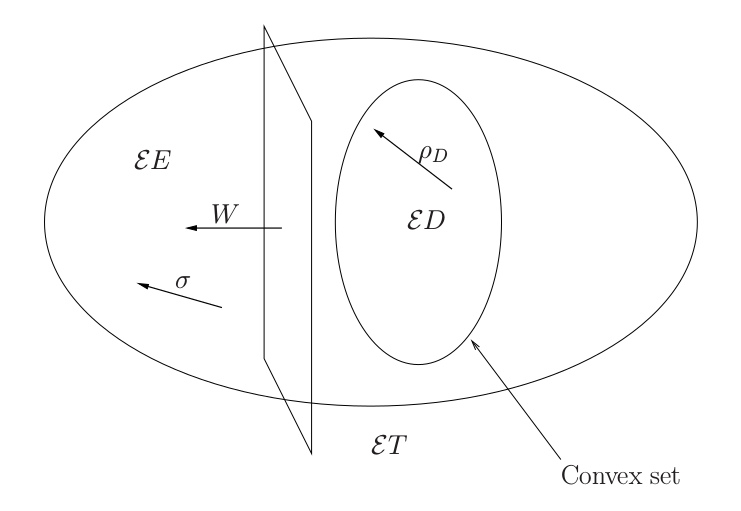
\includegraphics[scale=0.52]{figures/entanglementwitness.png}
    \caption{$D$ is the set of disentangled states and $E$ is the set of entangled states. If there exists a Hermitian operator $W$ which defines a plane between the two sets, then $W$ is called an entanglement witness.\newline Image courtesy of Vlatko Vedral, \textit{Introduction to Quantum Information Science} \cite{vedralqitbook}}
    \label{fig: Entanglement Witnesses}
  \end{center}
\end{figure}
\par To define the witness $W$, first consider an arbitrary vector space $V$. A plane in $V$ is specified by the vectors $\ket{\psi}$ such that
\begin{align*}
\braket{w \mid \psi} = 0
\end{align*}
where $w$ is a unit vector orthogonal to the plane.
\par Hermitian operators can also be thought of as vectors and an inner product can be defined for them as
\begin{align*}
\braket{O_1 \mid O_2} = tr \left( O_1^{\dagger} O_2 \right)
\end{align*}
For a Hermitian operator, that will become
\begin{align*}
\braket{O_1 \mid O_2} = tr \left( O_1 O_2 \right)
\end{align*}
Using this inner product, we can define a plane in the space of Hermitian operators $\tau$,
\begin{align*}
tr ( w \rho ) = 0
\end{align*}
The term on the right side can be a non-zero constant but we choose zero by convention.
\par Now suppose we have an entangled state $\sigma$. Then by our reasoning so far there exists a plane defined by a Hermitian operator $W$ such that $\sigma$ resides on one side and the convex set of all disentangled states resides on the other side. The points on the plane are defined by
\begin{align*}
tr ( \rho W ) = 0
\end{align*}
\par For each disentangled state $\rho_D$ we can either have $tr (\rho_D W) \geq 0$ or $tr (\rho_D W) \leq 0$. We choose $W$ such that $tr (\rho_D W) \geq 0$. Then for all entangled states $\sigma$ on the other side of the plane, $tr (\sigma W) < 0$.
\par Thus our test for entanglement becomes:
\begin{align*}
  tr (\sigma W) < 0 &\rightarrow \sigma \text{ is entangled} \\
  tr (\rho_D W) \geq 0 &\rightarrow \rho_D \text{ is disentangled}
\end{align*}
\par Whenever an entangled state exists an entanglement witness will also exist. Although in practice they can be hard to find. In the case of two qubits, entanglement witnesses are relatively easier to find. As the dimensionality of the system becomes larger, the search becomes harder and harder. \cite{vedralqitbook}

\subsection{The Peres-Horodecki criterion}
The Peres-Horodecki criterion is a reliable test of whether or not a bipartite state is entangled. The test proceeds as follows:
\begin{enumerate}
  \item Take a partial transpose of the density matrix.
  \item If the resultant matrix has a negative eigenvalue, then the state is entangled. Otherwise, the state is separable. (Reminder: A valid density matrix always has eigenvalues $\geq 0$)
\end{enumerate}
\par To calculate the partial transpose of the density matrix, we start by writing the basis states of qubit $A$ as $\ket{i}$ and $\ket{j}$ and the basis states of $B$ as $\ket{k}$ and $\ket{l}$. The density operator of the full system then is
\begin{align*}
\rho = \sum_{ijkl} p_{ijkl} \ket{i} \bra{j} \otimes \ket{k} \bra{l}
\end{align*}
The partial transpose with respect to $B$ will be
\begin{align*}
\left( \ket{k} \bra{l} \right)^T = \ket{l} \bra{k}
\end{align*}
By applying this transformation to the density operator, we get the partial transpose of that density operator.
\begin{align*}
\rho^{T_B} = (I \otimes T) \rho = \sum_{ijkl} p_{ijkl} \ket{i} \bra{j} \otimes \ket{l} \bra{k}
\end{align*}
\par After calculating the eigenvalues of this resultant matrix, if we find a negative eigenvalue then the state is entangled. If all the eigenvalues are zero or positive then the state is separable. \cite{vedralteleportation}

\section{Quantifying Quantum Entanglement}
\par We have seen that there are states that are entangled and states that are disentangled. Now let us go into a little more detail on the subject and ask the question of how to quantify the degree of entanglement contained in a given system. That is, measuring \textquotedblleft how much\textquotedblright\  entanglement is contained within a system. It turns out that we can also concentrate entanglement from a number of partially entangled states to form a smaller number of maximally entangled states.
\par We first specify the \textbf{desirable properties} that any \textquoteleft decent\textquoteright\ measure of entanglement should have. \cite{vedralteleportation}
\begin{enumerate}
  \item For any separable state $\rho$ the measure of entanglement should be zero.
        \begin{align*} E(\rho) = 0 \end{align*}
  \item A local unitary transformation, which is a unitary transformation of the form $U_A \otimes U_B$ and represents a change of basis, should not change the amount of entanglement in a state.
        \begin{align*} E(\rho) = E(U_A \otimes U_B \rho U_A^{\dagger} \otimes U_B^{\dagger}) \end{align*}
  \item Local operations \& classical communication (LOCC) - the act of classically communicating the results of local operations on the subsystems - and sub-selection cannot increase the expected entanglement \cite{vedralteleportation}. If we start with an ensemble in state $\rho$ and end up with sub-ensembles in states $\rho_i$ occurring with probabilities $p_i$, then
        \begin{align*} E(\rho) \geq \sum_i p_i E(\rho_i) \end{align*}
  \item Given two pairs of entangled particles in total state $\rho = \rho_1 \otimes \rho_2$, their entanglement is additive.
        \begin{align*} E(\rho) = E(\rho_1) + E(\rho_2) \end{align*}
\end{enumerate}
\par Now we shall look at some actual measures of entanglement which fulfill these requirements to be \textquoteleft decent\textquoteright\  entanglement measures. \cite{plenioentanglementmeasures}

\subsection{Entropy of Entanglement}
\par The entropy of entanglement is, in simple terms, the von Neumann entropy of the reduced density matrix of the given pure state.
\begin{align*}
S(\rho_A) = - tr \{ \rho_A \log \rho_A \}
\end{align*}
where $\rho_A$ is the reduced density matrix for subsystem $A$, obtained by tracing out subsystem $B$. That is, $\rho_A = tr_B \{\rho_{AB}\}$.
\par Entropy of entanglement suffers from the limitation that it only works as a good measure of entanglement for pure states. It does not work when mixed states are involved.

\subsection{Linear Entropy of Entanglement}
\par Linear entropy of entanglement is a linear approximation to the entropy of entanglement, in the same way that linear entropy is the linear approximation to von Neumann entropy. It is easier to calculate than the entropy of entanglement. The basic idea is the same: tracing out subsystem $B$ to obtain the reduced density matrix for subsystem $A$ and then taking its linear entropy.
\begin{align*}
S_L(\rho_A) = 1 - tr(\rho_A^2)
\end{align*}
\par This measure also suffers from the same problem as the entropy of entanglement. It does not work for mixed states. It can only work as a decent entanglement measure for pure states.

\subsection{Renyi Entanglement Entropy}
Renyi entanglement entropy of a density matrix $\rho$ is also defined in terms of its reduce density matrix $\rho_A$ or $\rho_B$.
\begin{align*}
S_\alpha (\rho_A) &= \frac{1}{1-\alpha} \log (tr\{\rho_A^\alpha\}) , \quad \alpha \neq 1 \: \text{and} \: \alpha > 0
\end{align*}
In terms of the eigenvalues of the reduced density matrix $q_i$,
\begin{align*}
S_\alpha (\rho_A) &= \frac{1}{1-\alpha} \log \left( \sum_i q_i^\alpha \right)
\end{align*}
where $\alpha$ is the Renyi index.
\par In the limit $\alpha \rightarrow 1$ it approaches the von Neumann entropy.

\subsection{Negativity}
\par Peres-Horodecki criterion tests for entanglement by presence of negative eigenvalues under partial transpose. Negativity is a measure of how negative the resulting matrix is. Mathematically, it is defined as
\begin{align*}
N(\rho) = \frac{\lVert \rho^{T_A} \rVert_1 - 1}{2}
\end{align*}
where $\rho^{T_A}$ is the partial transpose of the density matrix with respect to $A$ and $\lVert . \rVert_1$ denotes the trace norm.
\par Negativity has the property of non-increase under LOCC. But it does not have the additivity property. This brings us to logarithmic negativity.

\subsection{Logarithmic Negativity}
\par The logarithmic negativity of a bipartite state is
\begin{align*}
E_N(\rho) = log_2 \lVert \rho^{T_A} \rVert_1
\end{align*}
\par Logarithmic negativity is additive and provides an upper bound on how much entanglement can be distilled from a system.

\subsection{Concurrence}
\par Concurrence of a bipartite state $\rho$ is defined as
\begin{align*}
C(\rho) = max(0, \lambda_1 - \lambda_2 - \lambda_3 - \lambda_4)
\end{align*}
i.e. the greater one of these two quantities. The numbers $\lambda_1 > \lambda_2 > \lambda_3 > \lambda_4$ are eigenvalues of the Hermitian matrix
\begin{align*}
R = \sqrt{ \sqrt{\rho} \tilde{\rho} \sqrt{\rho} }
\end{align*}
in which
\begin{align*}
\tilde{\rho} = ( \sigma_y \otimes \sigma_y ) \rho^* ( \sigma_y \otimes \sigma_y )
\end{align*}
where $\rho^*$ is the complex conjugate of $\rho$ and $\sigma_y$ is the Pauli spin matrix known by the same label.
\par The value of concurrence ranges from 0 to 1. It is 0 for separable states and 1 for the maximally entangled state.
\par For multipartite states, concurrence takes on a more complicated form than the one shown here.

\subsection{Relative Entropy of Entanglement}
\par The basic idea for relative entropy of entanglement is based on distinguishability and geometrical distance. In this approach, when given a state $\sigma$, we compare its distance to each state from the whole set of disentangled states $D$ and pick the state $\rho$ which has the minimum distance from $\sigma$. The relative entropy of entanglement is thus this minimum distance.

\begin{align*}
E_{RE}(\sigma) = \underset{\rho \in D}{\min}  D(\sigma||\rho)
\end{align*}

\begin{figure}[h]
  \begin{center}
    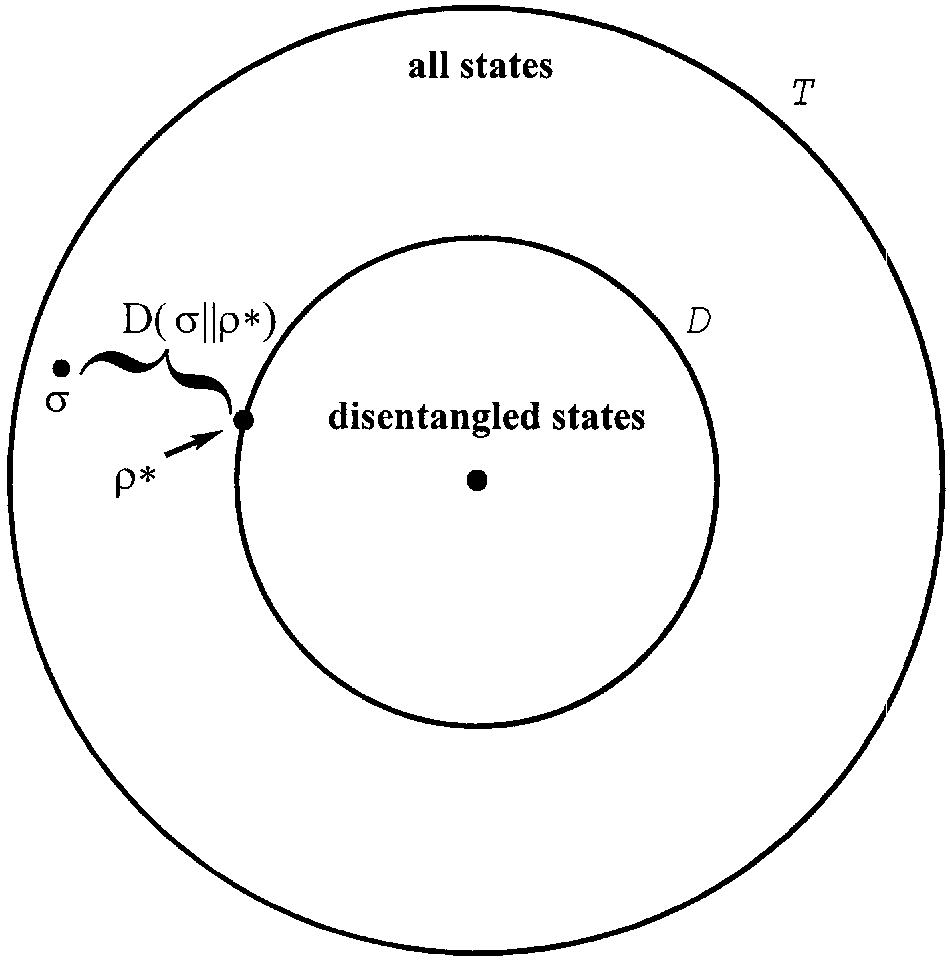
\includegraphics[scale=0.25]{figures/entanglement-distance.png}
    \caption{Relative entropy of entanglement: the distance from the nearest disentangled state\newline $\sigma$ is the state for which the quantity is to be measured. Over the whole state of disentangled states $\{\rho\}$, the state $\rho^*$ has the minimum distance from $\sigma$. The distance to $\rho^*$ is the relative entropy of entanglement of $\sigma$.\newline Image courtesy of Vlatko Vedral, \textit{Introduction to Quantum Information Science} \cite{vedralqitbook}}
    \label{fig: Relative Entropy of Entanglement}
  \end{center}
\end{figure}

\par Here the function $D$ is a measure of separation between the two density matrices. There are a number of separation measures available to define the \textquoteleft distance\textquoteright \  between two density matrices. Though it should be noted that not all distance measures will generate a \textquoteleft decent\textquoteright \  entanglement measure by our criteria. Those requirements have to be kept in mind when looking for an entanglement measure.

\par One distance measure which generates an entanglement measure satisfying the \textquoteleft decency\textquoteright \  criteria is the Kullback-Leibler distance - alternatively known as the relative entropy - that we talked about in section 3.5.2.
\begin{align*}
S(\sigma||\rho) &= tr \{ \sigma \log \sigma - \sigma \log \rho \}
\end{align*}
\par We can plug this into the formula for relative entropy of entanglement to generate an entanglement measure. We can similarly use many other distance measures in place of the Kullback-Leibler distance.
\par Relative entropy of entanglement is an important quantity because we can plug in various distance measures in place of the distance function $D$ and so we can derive many other entanglement measures from it - provided that they satisfy the criteria for decent entanglement measures. \cite{vedralteleportation}

